\chapter{Risk management}
\section{Definizione del rischio}
\begin{definizione}
    Il \textbf{risk management} è la disciplina che si occupa di identificare,
    gestire e potenzialmente eliminare i rischi prima che questi diventino un
    problema per il successo del progetto.
\end{definizione}
\begin{definizione}
    Definiamo \textbf{rischio} come la possibilità che ci sia un danno.
\end{definizione}
\begin{definizione}
    Definiamo \textbf{risk exposure}, che è una grandezza, per calcolare quanto
    un progetto sia esposto ad un rischio. Viene calcolato come:
    \begin{equation}
        RE = P(UO) \cdot L(UO)
    \end{equation}
    dove:
    \begin{itemize}
        \item $P(UO)$: è la probabilità di un unsatisfactory outcome, ovvero la
              probabilità che effettivamente un danno sia prodotto.
        \item $L(UO)$: è l'entità del danno stesso, ovvero è la perdita per le
              parti interessate se il risultato non è soddisfacente.
    \end{itemize}

    Tanto più un rischio è probabile e tanto più il rischio crea un danno, di
    conseguenza cresce il risk exposure.
\end{definizione}
\begin{definizione}
    Definiamo \textbf{outcome unsatisfactory} come un risultato non positivo che
    riguarda diverse aree:
    \begin{itemize}
        \item L'area relativa all'esperienza degli utenti, con un progetto che
              presenta le funzionalità sbagliate. In questo caso se i problemi sono
              gravi si hanno alti rischi che portano al fallimento del prodotto.
        \item L'area relativa agli sviluppatori, con rischi che possono riguardare
              superamento del budget oppure prolungamenti delle deadlines.
        \item L'area riguardante i manutentori, con rischi che impattano nella
              qualità bassa di software e hardware.
    \end{itemize}
\end{definizione}

Se abbiamo un rischio che produce un outcome unsatisfactory il primo elemento su
cui soffermarsi è lo studio degli eventi che abilitano il rischio, detti \textbf{risk triggers}.

Possiamo distinguere due principali classi di rischio:
\begin{enumerate}
    \item \textbf{Process-related risks}: rappresenti rischi con impatto
          negativo sul processo e sugli obiettivi di sviluppo.
    \item \textbf{Product-related risks}: rappresenti rischi con impatto sul
          prodotto e su obiettivi del sistema funzionali o meno, come fallimenti
          riguardanti la qualità del prodotto o la distribuzione dello stesso.
\end{enumerate}
Entrambe le classi possono portare al fallimento del progetto e quindi vanno gestite
entrambe.
\section{Risk Management}
Bisogna quindi imparare a gestire i rischi. Per fare ciò si utilizza un processo
strutturato in due fasi:
\begin{enumerate}
    \item \textbf{Risk Assessment}: in questa fase si vanno a valutare i rischi
          attraverso:
          \begin{itemize}
              \item \textbf{Risk Identification}: ovvero una fase di identificazione
                    dei rischi.
              \item \textbf{Risk Analysis}: ovvero l'analisi dei rischi identificati
                    nella fase precedente tramite calcolo del \textit{risk exposure} e
                    studio dei \textit{triggers}.
              \item \textbf{Risk Prioritization}: ovvero si vanno a definire delle
                    priorità nei rischi analizzati, in modo da concentrarsi sui più
                    pericolosi per poi passare a quelli meno pericolosi.
          \end{itemize}

          Alla fine di questa fase, si produce una lista ordinata sulla pericolosità
          dei rischi.
    \item \textbf{Risk Control} e consiste nel risk management planning, producendo
          piani di controllo di due tipi:
          \begin{enumerate}
              \item \textbf{Piani di management}: per la gestione del rischio prima che
                    si verifichi.
              \item \textbf{Piani di contingency}: per il contenimento di rischi divenuti
                    realtà qualora il piano di management fallisca, sapendo cosa fare a priori
                    in caso di emergenza.
          \end{enumerate}

          Si hanno quindi due sotto-fasi per i due tipi di piani:
          \begin{enumerate}
              \item \textbf{Risk monitoring}.
              \item \textbf{Risk resolution}.
          \end{enumerate}
\end{enumerate}

Queste due fasi vengono ciclicamente ripetute durante il ciclo di vita dello sviluppo di un software.
\subsection{Risk identification}
In questa fase, si studia come identificare i rischi. Tale operazione è legata
alle competenze degli analisti. Un modo comune di realizzare questa operazione è
mediante l'uso delle check-list, liste che includono un insieme di rischi plausibili
comuni a molti progetti. L'analista scorre tale lista cercando rischi che possono
essere applicati al progetto in analisi.

Alcuni rischi possono verificarsi sempre ma va preso in considerazione solo per
motivi specifici identificabili nel mio progetto. Si hanno altri metodi per identificare i rischi:
\begin{itemize}
    \item Riunioni di confronto, brainstorming e workshop.
    \item Confronto con altre organizzazioni e con altri prodotti.
\end{itemize}
\subsection{Risk analysis}
L'analisi dei rischi viene realizzata sfruttando l'esperienza e valutando le
reali probabilità che un rischio diventi reale. Come per la fase precedente, si
hanno degli schemi su cui basarsi, come modelli di stima dei costi, modelli delle
prestazioni, basati su simulazioni, prototipi, analogie con altri progetti e
check-list. Le stime sono molto specifiche sul singolo progetto.

L'analisi dei rischi può anche comportare lo studio delle decisioni da prendere
al fine di minimizzare il risk exposure, scegliendo o meno tra varie opzioni,
scegliendo in modo guidato dai rischi. A tal fine si usano i \textbf{decision tree}
nei quali la radice rappresenta il problema.

Si hanno di volta in volta i vari scenari, con le stime di probabilità di trovare
un errore critico, di fallimento, di non trovare errori critici e così via. Tali
probabilità verranno usate per il calcolo del risk exposure insieme ad un
quantificatore di $L(UO)$ spesso pari all'effettivo costo che conseguirebbe al
risultato ottenuto. Infine i vari risk exposure di ogni caso vengono sommati per
ottenere il risk exposure finale. Si può fare un'\textbf{analisi di sensitività}
cambiando le percentuali o i costi al fine di ottenere un certo risultato, in
modo da capire come si dovrebbe comportare.
\begin{esempio}[Decision tree]
    Vediamo ora un esempio di come utilizzare un albero di decisione per effettuare
    l'analisi di un rischio figura \ref{fig:tree}.
    \begin{figure}[!ht]
        \centering
        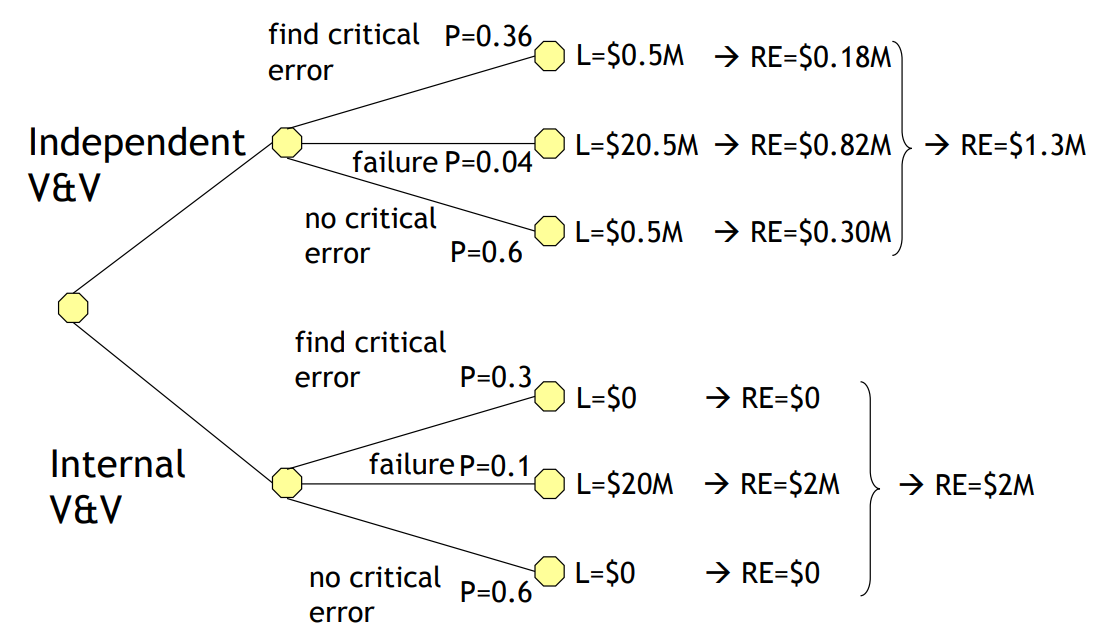
\includegraphics[width=0.6\textwidth]{img/risk/tree.png}
        \caption{Decision tree}
        \label{fig:tree}
    \end{figure}
\end{esempio}

Ragionando sulle cause dei rischi usiamo il cosiddetto risk tree. Questo albero
ha come radice il rischio. Ogni nodo, detto failure node, è un evento che si può
scomporre in altri eventi, fino alle foglie. La scomposizione è guidata da due
tipi di nodi link:
\begin{enumerate}
    \item \textbf{and-node}: dove i figli di tali nodi sono eventi legati dal un and.
    \item \textbf{or-node}: dove i figli di tali nodi sono eventi legati dal un or.
\end{enumerate}
\begin{esempio}[Risk tree]
    Vediamo ora un esempio di risk tree figura \ref{fig:risk-tree}.
    \begin{figure}[!ht]
        \centering
        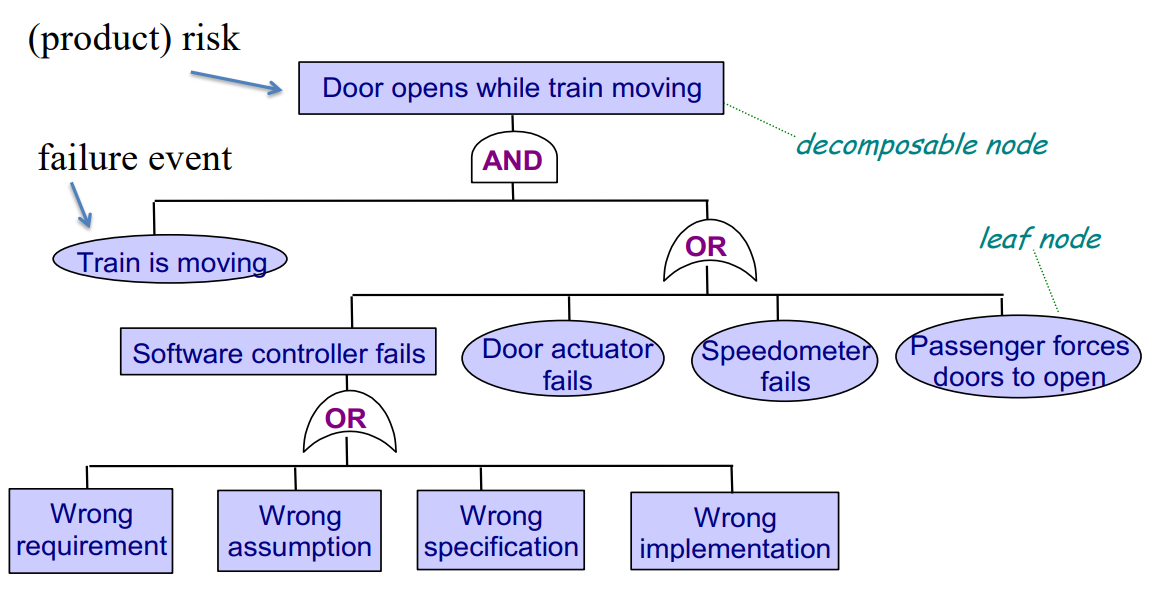
\includegraphics[width=0.6\textwidth]{img/risk/risktree.png}
        \caption{Risk tree}
        \label{fig:risk-tree}
    \end{figure}
\end{esempio}
Nodi And/Or vengono rappresentati tramite i simboli delle porte logiche. Dato un
risk tree cerco le combinazioni di eventi atomici che possono portare al rischio.
Per farlo si esegue la cut-set tree derivation, ovvero, partendo dalla radice, si
riporta in ogni nodo la combinazione di eventi che possono produrre il fallimento
e si vanno a calcolare le varie combinazioni degli eventi foglia. Praticamente si
deriva un insieme di eventi non scomponibili sulle combinazioni dell'and.
\subsection{Risk prioritization}
Bisogna capire quali rischi sono più importanti di altri. Per farlo si pongono i
valori di $P(UO)$ e $L(UO)$ in un range, per esempio, da 1 a 10, ricalcolando il
risk exposure. Una volta fatto si lavora in base al risk-exposure.

Si procede disegnando i dati su un piano con $P(UO)$ sull'asse delle y e $L(UO)$
su quello delle x e posizionad gli eventi su tale piano. Qualora i valori siano
in un range si rappresentano con un segmento tra i due valori limite di risk exposure.
Una volta rappresentati gli eventi, posso utilizzare delle curve per identificare
zone di rischio diverse in base al risk exposure in modo da classificare i vari eventi.
\subsection{Risk control}
Bisogna quindi capire come gestire i rischi. Per ogni rischio bisogna definire e
documentare un piano specifico indicante:
\begin{itemize}
    \item Cosa si sta gestendo.
    \item Come mitigare il rischio e quando farlo.
    \item Di chi è la responsabilità.
    \item Come approcciarsi al rischio.
    \item Il costo dell'approccio al rischio.
\end{itemize}

Anche in questo caso ci vengono incontro liste e check-list con le tecniche di risk
management più comuni in base al rischio specifico. Ci sono comunque strategie generali:
\begin{itemize}
    \item Lavorare sulla probabilità che il rischio avvenga, sulla probabilità dei
          triggers. Bisogna capire come diminuire la probabilità.
    \item Lavorare sull'eliminazione stessa del rischio.
    \item Lavorare sulla riduzione della probabilità di avere conseguenze al danno,
          non viene quindi ridotto il rischio.
    \item Lavorare sull'eliminazione stessa del danno conseguente al rischio.
    \item Lavorare sul mitigare le conseguenze di un rischio, diminuendo l'entità
          del danno.
\end{itemize}

Bisogna anche studiare le \textbf{contromisure}, da scegliere e attivare in base
alla situazione. Si hanno due metodi quantitativi principali per ragionare
quantitativamente sulle contromisure:
\begin{enumerate}
    \item \textbf{Risk-reduction leverage}: dove si calcola quanto una certa
          contromisura può ridurre un certo rischio, utilizzando la seguente formula:
          \begin{equation}
              RRL(r, cm) = \frac{RE(r) - RE(\frac{r}{cm})}{const(cm)}
          \end{equation}
          dove $r$ rappresenta il rischio, $cm$ la contromisura e $\frac{r}{cm}$ la
          contromisura $cm$ applicata al rischio $r$.

          Calcolo quindi la differenza di risk exposure avendo e non avendo la contromisura
          e la divido per il costo della contromisura. La miglior contromisura è quella
          con il RRL maggiore, avendo minor costo e maggior efficacia dal punto di vista
          del risk exposure.
    \item \textbf{Defect detection prevention}: questo metodo confronta le varie
          contromisure, confrontando anche gli obiettivi del progetto, in modo quantitativo
          facendo un confronto indiretto, producendo matrici in cui si ragiona in modo
          indipendente sulle singole contromisure e sui singoli rischi ma confrontando
          anche in modo multiplo.

          Si ha un ciclo a tre step:
          \begin{enumerate}
              \item \textbf{Elaborare la matrice di impatto dei rischi} (\textit{risk
                        impact matrix}): questa matrice calcola l'impatto dei rischi sugli obiettivi
                    del progetto. I valori della matrice variano da 0, nessun impatto, a 1,
                    completa perdita di soddisfazione. Ogni rischio viene accompagnato dalla
                    probabilità $P$ che accada. Ogni obiettivo è accompagnato dal peso $W$
                    che ha nel progetto.

                    La \textbf{criticità} di un rischio rispetto a tutti gli obiettivi indicati:
                    \begin{equation}
                        \text{criticality}(r) = P(r) \cdot \sum_{obj} (\text{impact}(r, obj) \cdot W(obj))
                    \end{equation}
                    La criticità sale se sale l'impatto e se sale la probabilità del rischio.
                    Un altro dato è la \textbf{perdita} di raggiungimento di un obiettivo
                    qualora tutti i rischi si verificassero:
                    \begin{equation}
                        loss(obj) = W(obj) \cdot \sum_{obj} (impact(r, obj) \cdot P(r))
                    \end{equation}
              \item \textbf{Elaborare contromisure efficaci per la matrice}: si usa il
                    fattore di criticità del rischio. Viene prodotta una nuova matrice con
                    colonne pari ai rischi e righe pari alle contromisure. I valori saranno
                    le riduzioni di rischio di una contromisura $cm$ sul rischio $r$. La
                    riduzione va da 0, nessuna riduzione, a 1, rischio eliminato.

                    Possiamo calcolare la \textbf{combineReduction}, che ci dice quanto un
                    rischio viene ridotto se tutte le contromisure sono attivate:
                    \begin{equation}
                        \text{combineReduction}(r) = 1 - \prod_{cm}(1 - \text{reduction}(cm, r))
                    \end{equation}
                    Un altro valore è l'\textbf{overallEffect}, ovvero l'effetto di ogni
                    contromisura sull'insieme dei rischi considerato:
                    \begin{equation}
                        \text{overalleffect}(cm) = \sum_{r} (\text{reduction}(cm; r) \cdot \text{criticality}(r))
                    \end{equation} si avrà effetto maggior riducendo rischi molto critici.
              \item \textbf{Determinare il bilanciamento migliore tra riduzione dei rischi e costo delle contromisure}.
                    Bisogna considerare anche il costo di ogni contromisure e quindi si fa il
                    rapporto tra effetto di ciascuna contromisura e il suo costo e scegliendo il migliore.
          \end{enumerate}
\end{enumerate}

Il \textbf{contingency plan} viene attuato qualora il rischio si traduca in realtà.
Si passa quindi al risk monitoring/resolution. Queste due parti sono tra loro
integrate. I rischi vanno monitorati e occorrenza vanno risolti il prima possibile.
Tutte queste attività sono costose e si lavora su un insieme limitato di rischi.